\documentclass{standalone}
\usepackage{tikz}
\usetikzlibrary{patterns, positioning}

\begin{document}
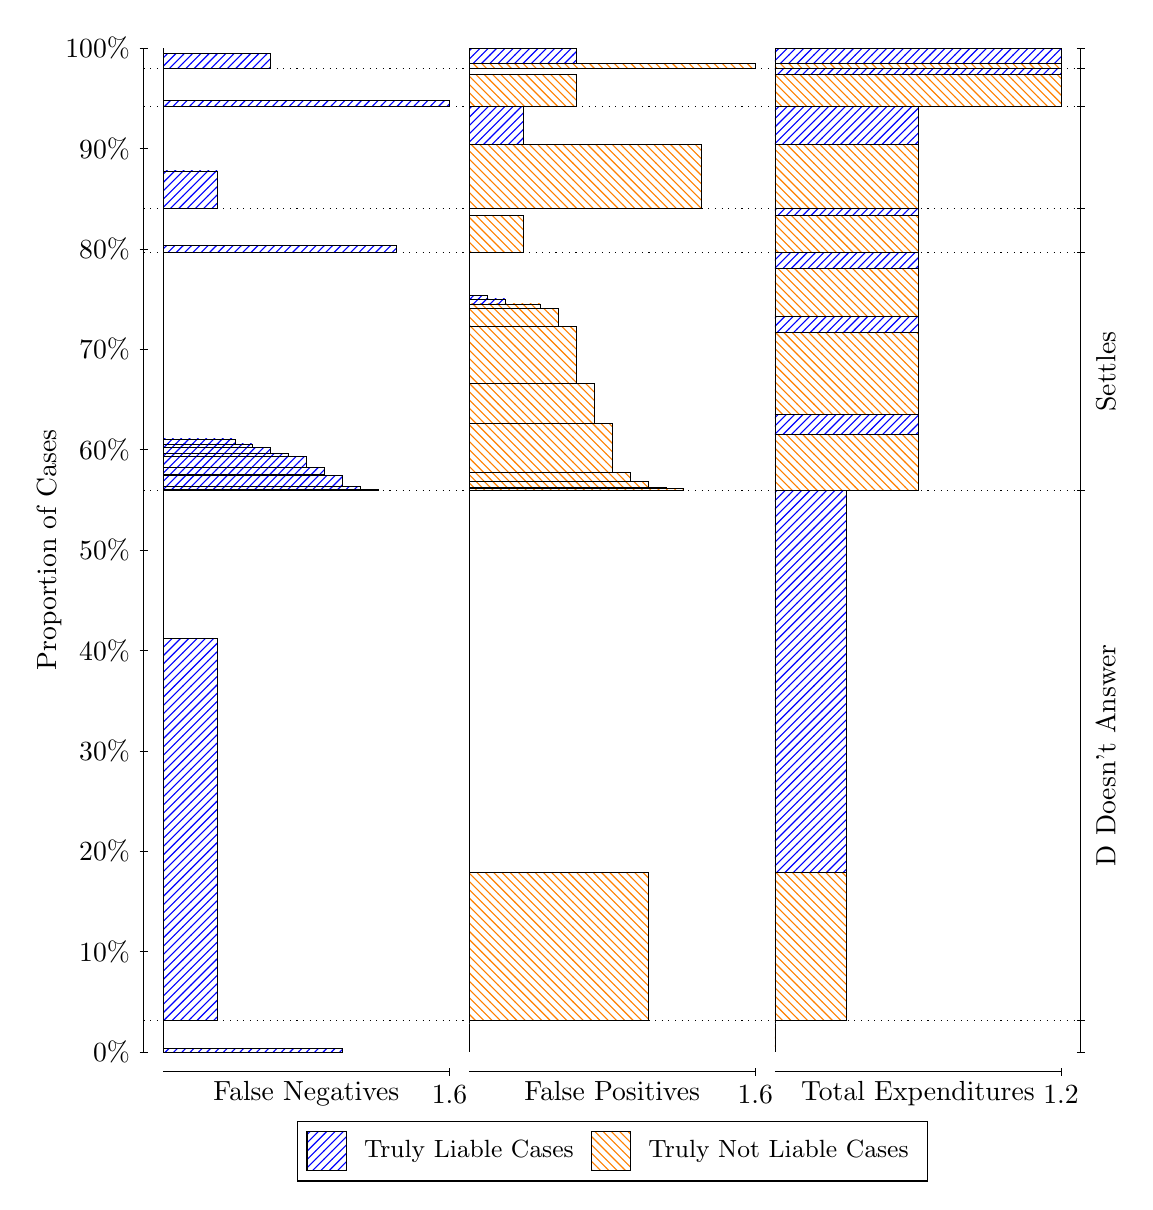
\begin{tikzpicture}
\draw[black, very thin] (1.5,1.75) -- (1.5,14.5);
\node[rotate=90, anchor=center] at (0.3, 8.125) {Proportion of Cases};
\draw[black, very thin] (1.45,1.75) -- (1.55,1.75);
\node[anchor=east] at (1.45, 1.75) {0\%};
\draw[black, very thin] (1.45,3.025) -- (1.55,3.025);
\node[anchor=east] at (1.45, 3.025) {10\%};
\draw[black, very thin] (1.45,4.3) -- (1.55,4.3);
\node[anchor=east] at (1.45, 4.3) {20\%};
\draw[black, very thin] (1.45,5.575) -- (1.55,5.575);
\node[anchor=east] at (1.45, 5.575) {30\%};
\draw[black, very thin] (1.45,6.85) -- (1.55,6.85);
\node[anchor=east] at (1.45, 6.85) {40\%};
\draw[black, very thin] (1.45,8.125) -- (1.55,8.125);
\node[anchor=east] at (1.45, 8.125) {50\%};
\draw[black, very thin] (1.45,9.4) -- (1.55,9.4);
\node[anchor=east] at (1.45, 9.4) {60\%};
\draw[black, very thin] (1.45,10.675) -- (1.55,10.675);
\node[anchor=east] at (1.45, 10.675) {70\%};
\draw[black, very thin] (1.45,11.95) -- (1.55,11.95);
\node[anchor=east] at (1.45, 11.95) {80\%};
\draw[black, very thin] (1.45,13.225) -- (1.55,13.225);
\node[anchor=east] at (1.45, 13.225) {90\%};
\draw[black, very thin] (1.45,14.5) -- (1.55,14.5);
\node[anchor=east] at (1.45, 14.5) {100\%};

\draw[black, very thin] (13.4,1.75) -- (13.4,14.5);
\draw[black, very thin] (13.35,1.75) -- (13.45,1.75);
\node[anchor=west] at (13.35, 1.75) {};
\draw[black, very thin] (13.35,2.1536) -- (13.45,2.1536);
\node[anchor=west] at (13.35, 2.1536) {};
\draw[black, very thin] (13.35,8.8821) -- (13.45,8.8821);
\node[anchor=west] at (13.35, 8.8821) {};
\draw[black, very thin] (13.35,11.905) -- (13.45,11.905);
\node[anchor=west] at (13.35, 11.905) {};
\draw[black, very thin] (13.35,12.461) -- (13.45,12.461);
\node[anchor=west] at (13.35, 12.461) {};
\draw[black, very thin] (13.35,13.76) -- (13.45,13.76);
\node[anchor=west] at (13.35, 13.76) {};
\draw[black, very thin] (13.35,14.239) -- (13.45,14.239);
\node[anchor=west] at (13.35, 14.239) {};
\draw[black, very thin] (13.35,14.5) -- (13.45,14.5);
\node[anchor=west] at (13.35, 14.5) {};

\draw[black, very thin, pattern color=blue, pattern=north east lines] (1.75,1.75) rectangle (4.0208,1.7925);
\draw[black, very thin, pattern color=orange, pattern=north west lines] (1.75,1.7925) rectangle (1.75,2.1536);
\draw[black, very thin, pattern color=blue, pattern=north east lines] (1.75,2.1536) rectangle (2.4312,7.0049);
\draw[black, very thin, pattern color=orange, pattern=north west lines] (1.75,7.0049) rectangle (1.75,8.8821);
\draw[black, very thin, pattern color=blue, pattern=north east lines] (1.75,8.8821) rectangle (4.475,8.8932);
\draw[black, very thin, pattern color=blue, pattern=north east lines] (1.75,8.8932) rectangle (4.2479,8.937);
\draw[black, very thin, pattern color=blue, pattern=north east lines] (1.75,8.937) rectangle (4.0208,9.0712);
\draw[black, very thin, pattern color=blue, pattern=north east lines] (1.75,9.0712) rectangle (3.7937,9.0836);
\draw[black, very thin, pattern color=blue, pattern=north east lines] (1.75,9.0836) rectangle (3.7937,9.1741);
\draw[black, very thin, pattern color=blue, pattern=north east lines] (1.75,9.1741) rectangle (3.5667,9.3092);
\draw[black, very thin, pattern color=blue, pattern=north east lines] (1.75,9.3092) rectangle (3.3396,9.3542);
\draw[black, very thin, pattern color=blue, pattern=north east lines] (1.75,9.3542) rectangle (3.1125,9.4298);
\draw[black, very thin, pattern color=blue, pattern=north east lines] (1.75,9.4298) rectangle (2.8854,9.4719);
\draw[black, very thin, pattern color=blue, pattern=north east lines] (1.75,9.4719) rectangle (2.6583,9.5365);
\draw[black, very thin, pattern color=orange, pattern=north west lines] (1.75,9.5365) rectangle (1.75,11.905);
\draw[black, very thin, pattern color=blue, pattern=north east lines] (1.75,11.905) rectangle (4.7021,11.989);
\draw[black, very thin, pattern color=orange, pattern=north west lines] (1.75,11.989) rectangle (1.75,12.461);
\draw[black, very thin, pattern color=blue, pattern=north east lines] (1.75,12.461) rectangle (2.4312,12.94);
\draw[black, very thin, pattern color=orange, pattern=north west lines] (1.75,12.94) rectangle (1.75,13.76);
\draw[black, very thin, pattern color=blue, pattern=north east lines] (1.75,13.76) rectangle (5.3833,13.831);
\draw[black, very thin, pattern color=orange, pattern=north west lines] (1.75,13.831) rectangle (1.75,14.239);
\draw[black, very thin, pattern color=blue, pattern=north east lines] (1.75,14.239) rectangle (3.1125,14.43);
\draw[black, very thin, pattern color=orange, pattern=north west lines] (1.75,14.43) rectangle (1.75,14.5);
\draw[black, very thin, pattern color=orange, pattern=north west lines] (5.6333,1.75) rectangle (5.6333,2.1111);
\draw[black, very thin, pattern color=blue, pattern=north east lines] (5.6333,2.1111) rectangle (5.6333,2.1536);
\draw[black, very thin, pattern color=orange, pattern=north west lines] (5.6333,2.1536) rectangle (7.9042,4.0307);
\draw[black, very thin, pattern color=blue, pattern=north east lines] (5.6333,4.0307) rectangle (5.6333,8.8821);
\draw[black, very thin, pattern color=orange, pattern=north west lines] (5.6333,8.8821) rectangle (8.3583,8.9052);
\draw[black, very thin, pattern color=orange, pattern=north west lines] (5.6333,8.9052) rectangle (8.1313,8.9249);
\draw[black, very thin, pattern color=orange, pattern=north west lines] (5.6333,8.9249) rectangle (7.9042,8.999);
\draw[black, very thin, pattern color=orange, pattern=north west lines] (5.6333,8.999) rectangle (7.6771,9.1093);
\draw[black, very thin, pattern color=orange, pattern=north west lines] (5.6333,9.1093) rectangle (7.45,9.7291);
\draw[black, very thin, pattern color=orange, pattern=north west lines] (5.6333,9.7291) rectangle (7.2229,10.24);
\draw[black, very thin, pattern color=orange, pattern=north west lines] (5.6333,10.24) rectangle (6.9958,10.96);
\draw[black, very thin, pattern color=orange, pattern=north west lines] (5.6333,10.96) rectangle (6.7687,11.197);
\draw[black, very thin, pattern color=orange, pattern=north west lines] (5.6333,11.197) rectangle (6.5417,11.25);
\draw[black, very thin, pattern color=blue, pattern=north east lines] (5.6333,11.25) rectangle (6.0875,11.315);
\draw[black, very thin, pattern color=blue, pattern=north east lines] (5.6333,11.315) rectangle (5.8604,11.357);
\draw[black, very thin, pattern color=blue, pattern=north east lines] (5.6333,11.357) rectangle (5.6333,11.905);
\draw[black, very thin, pattern color=orange, pattern=north west lines] (5.6333,11.905) rectangle (6.3146,12.376);
\draw[black, very thin, pattern color=blue, pattern=north east lines] (5.6333,12.376) rectangle (5.6333,12.461);
\draw[black, very thin, pattern color=orange, pattern=north west lines] (5.6333,12.461) rectangle (8.5854,13.28);
\draw[black, very thin, pattern color=blue, pattern=north east lines] (5.6333,13.28) rectangle (6.3146,13.76);
\draw[black, very thin, pattern color=orange, pattern=north west lines] (5.6333,13.76) rectangle (6.9958,14.167);
\draw[black, very thin, pattern color=blue, pattern=north east lines] (5.6333,14.167) rectangle (5.6333,14.239);
\draw[black, very thin, pattern color=orange, pattern=north west lines] (5.6333,14.239) rectangle (9.2667,14.309);
\draw[black, very thin, pattern color=blue, pattern=north east lines] (5.6333,14.309) rectangle (6.9958,14.5);
\draw[black, very thin, pattern color=orange, pattern=north west lines] (9.5167,1.75) rectangle (9.5167,2.1111);
\draw[black, very thin, pattern color=blue, pattern=north east lines] (9.5167,2.1111) rectangle (9.5167,2.1536);
\draw[black, very thin, pattern color=orange, pattern=north west lines] (9.5167,2.1536) rectangle (10.425,4.0307);
\draw[black, very thin, pattern color=blue, pattern=north east lines] (9.5167,4.0307) rectangle (10.425,8.8821);
\draw[black, very thin, pattern color=orange, pattern=north west lines] (9.5167,8.8821) rectangle (11.333,9.5957);
\draw[black, very thin, pattern color=blue, pattern=north east lines] (9.5167,9.5957) rectangle (11.333,9.8486);
\draw[black, very thin, pattern color=orange, pattern=north west lines] (9.5167,9.8486) rectangle (11.333,10.891);
\draw[black, very thin, pattern color=blue, pattern=north east lines] (9.5167,10.891) rectangle (11.333,11.093);
\draw[black, very thin, pattern color=orange, pattern=north west lines] (9.5167,11.093) rectangle (11.333,11.704);
\draw[black, very thin, pattern color=blue, pattern=north east lines] (9.5167,11.704) rectangle (11.333,11.905);
\draw[black, very thin, pattern color=orange, pattern=north west lines] (9.5167,11.905) rectangle (11.333,12.376);
\draw[black, very thin, pattern color=blue, pattern=north east lines] (9.5167,12.376) rectangle (11.333,12.461);
\draw[black, very thin, pattern color=orange, pattern=north west lines] (9.5167,12.461) rectangle (11.333,13.28);
\draw[black, very thin, pattern color=blue, pattern=north east lines] (9.5167,13.28) rectangle (11.333,13.76);
\draw[black, very thin, pattern color=orange, pattern=north west lines] (9.5167,13.76) rectangle (13.15,14.167);
\draw[black, very thin, pattern color=blue, pattern=north east lines] (9.5167,14.167) rectangle (13.15,14.239);
\draw[black, very thin, pattern color=orange, pattern=north west lines] (9.5167,14.239) rectangle (13.15,14.309);
\draw[black, very thin, pattern color=blue, pattern=north east lines] (9.5167,14.309) rectangle (13.15,14.5);
\draw[black, dotted] (1.5,2.1536) -- (13.4,2.1536);
\draw[black, dotted] (1.5,8.8821) -- (13.4,8.8821);
\draw[black, dotted] (1.5,11.905) -- (13.4,11.905);
\draw[black, dotted] (1.5,12.461) -- (13.4,12.461);
\draw[black, dotted] (1.5,13.76) -- (13.4,13.76);
\draw[black, dotted] (1.5,14.239) -- (13.4,14.239);
\draw[black, very thin] (1.75,1.5) -- (5.3833,1.5);
\node[anchor=north] at (3.5667, 1.5) {False Negatives};
\draw[black, very thin] (5.3833,1.45) -- (5.3833,1.55);
\node[anchor=north] at (5.3833, 1.45) {1.6};

\draw[black, very thin] (5.6333,1.5) -- (9.2667,1.5);
\node[anchor=north] at (7.45, 1.5) {False Positives};
\draw[black, very thin] (9.2667,1.45) -- (9.2667,1.55);
\node[anchor=north] at (9.2667, 1.45) {1.6};

\draw[black, very thin] (9.5167,1.5) -- (13.15,1.5);
\node[anchor=north] at (11.333, 1.5) {Total Expenditures};
\draw[black, very thin] (13.15,1.45) -- (13.15,1.55);
\node[anchor=north] at (13.15, 1.45) {1.2};


\node[black, centered, rotate=90] at (13.72, 5.5178) {D Doesn't Answer};
\node[black, centered, rotate=90] at (13.72, 10.393) {Settles};





\draw (7.449999999999999,1.5) node[draw=none] (baseCoordinate) {};
\begin{scope}[align=center]
        \matrix[scale=0.5, draw=black, below=0.5cm of baseCoordinate, nodes={draw}, column sep=0.1cm]{
            \node[rectangle, draw, minimum width=0.5cm, minimum height=0.5cm, pattern=north east lines, pattern color=blue] {}; &
            \node[draw=none, font=\small] (B) {Truly Liable Cases}; &
            \node[rectangle, draw, minimum width=0.5cm, minimum height=0.5cm, pattern=north west lines, pattern color=orange] {}; &
            \node[draw=none, font=\small] (B) {Truly Not Liable Cases}; \\
            };
\end{scope}

\end{tikzpicture}
\end{document}